\documentclass[12pt]{article}
\usepackage[english]{babel}
\usepackage[numbers]{natbib}
\usepackage{graphicx}
\usepackage{xcolor}
\usepackage{sectsty}
\usepackage{float}
\bibliographystyle{apalike}
\setcitestyle{open={[},close={]}}
\sectionfont{\color{DarkBlue}} 
\subsectionfont{\color{LightBlue}}
\subsubsectionfont{\color{LightBlue}}
\paragraphfont{\color{LightBlue}}
\subparagraphfont{\color{LightBlue}}
\begin{document}
\definecolor{DarkBlue}{HTML}{4a5a8a}
\definecolor{LightBlue}{HTML}{4f81bf}
\begin{titlepage}
\begin{flushleft}
\vspace*{1cm}
\Huge
\textbf{Cretaceous Gardens Controller}\\
\vspace{1cm}
\Huge
\textit{Requirements Definition Document}\\
\vspace{1cm}
\Large
\textit{RDD Version 1.0}\\
\vspace{5cm}
\LARGE
Team \#3\\
17 October 2019
\vfill
\Huge
\textbf{CS 460 Software Engineering}
\end{flushleft}
\end{titlepage}
\normalsize
\tableofcontents
\newpage
\section{Introduction} %Zeke

\section{Definition of Terms} %Zeke
\label{def}
\textit{This section details all terms used in the document for the sake of minimizing ambiguity as much as possible among team members, between teams, and between the client and the team. Remaining with the interest of preserving the integrity to our communication, the following terms may be altered, reduced, or augmented to better reflect what it is that everyone is attempting to say.}
% the basis for accurate communication
\pagebreak
	

\section{Objectives} 
\label{obj}
\paragraph{} \textit{We came up with four main objectives\footnote{Objectives by Anas and Siri.} that we believe are critical to this specific system. We believe if we design the software around these objectives that it will produce the best  and most appropriate product.}
\subsection{Safety}\label{saf}
\paragraph{}The main objective of this product is to build a CGCS which focuses on safe and reliable experience to our customers. Whether we talk about the electric fences or self-driving cars, ensuring safety is the highest priority. We want the visitors to feel safe in every way possible and therefore, all these necessary measurements are taken into account by the CGCS.
\subsection{User Experience}\label{use}
\paragraph{}We want the user to have an amazing experience. Since this is a park to witness the amazing T-Rex, the user experience should be top notch. We will achieve this by focusing on the details of every interaction with the user. This involves easy token purchases and intuitive interaction with the vehicles. The user experience must be reliable. 
\subsection{Maintainability}\label{mai}
\paragraph{}The entire CGCS and all nodes that it controls will be designed with maintainability in mind. The system will understand the state of its health and report on it. Every node of the system will be designed this way and the CGCS will understand the health state of all systems. The system will have redundant infrastructure to maintain the system with minimal downtime specifically focus on the electric fence.
\subsection{Efficiency}\label{eff}
\paragraph{}When it comes to efficiency, the CGCS will make sure that both the software and hardware components are highly efficient and functional. Whether we talk about self-driving cars, pay kiosks, camera system, gps, or electric fences, the CGCS must be efficient in interacting with them. This will be possible when all the other objectives are met.  



\section{Overall System Organization} 
\label{sys}
\paragraph{} The CGCS will be the centralized system\footnote{System Organization by Anas and Siri.} and it will manage all the other associated components. Figure 1 shows the black box diagram of CGCS. The CGCS receives inputs from the sensors as well as user interfaces and emergency systems such as Global Alarm System and responds to them through appropriate output actions as described below in the diagram. 

    \begin{figure}[H]
  		\centerline{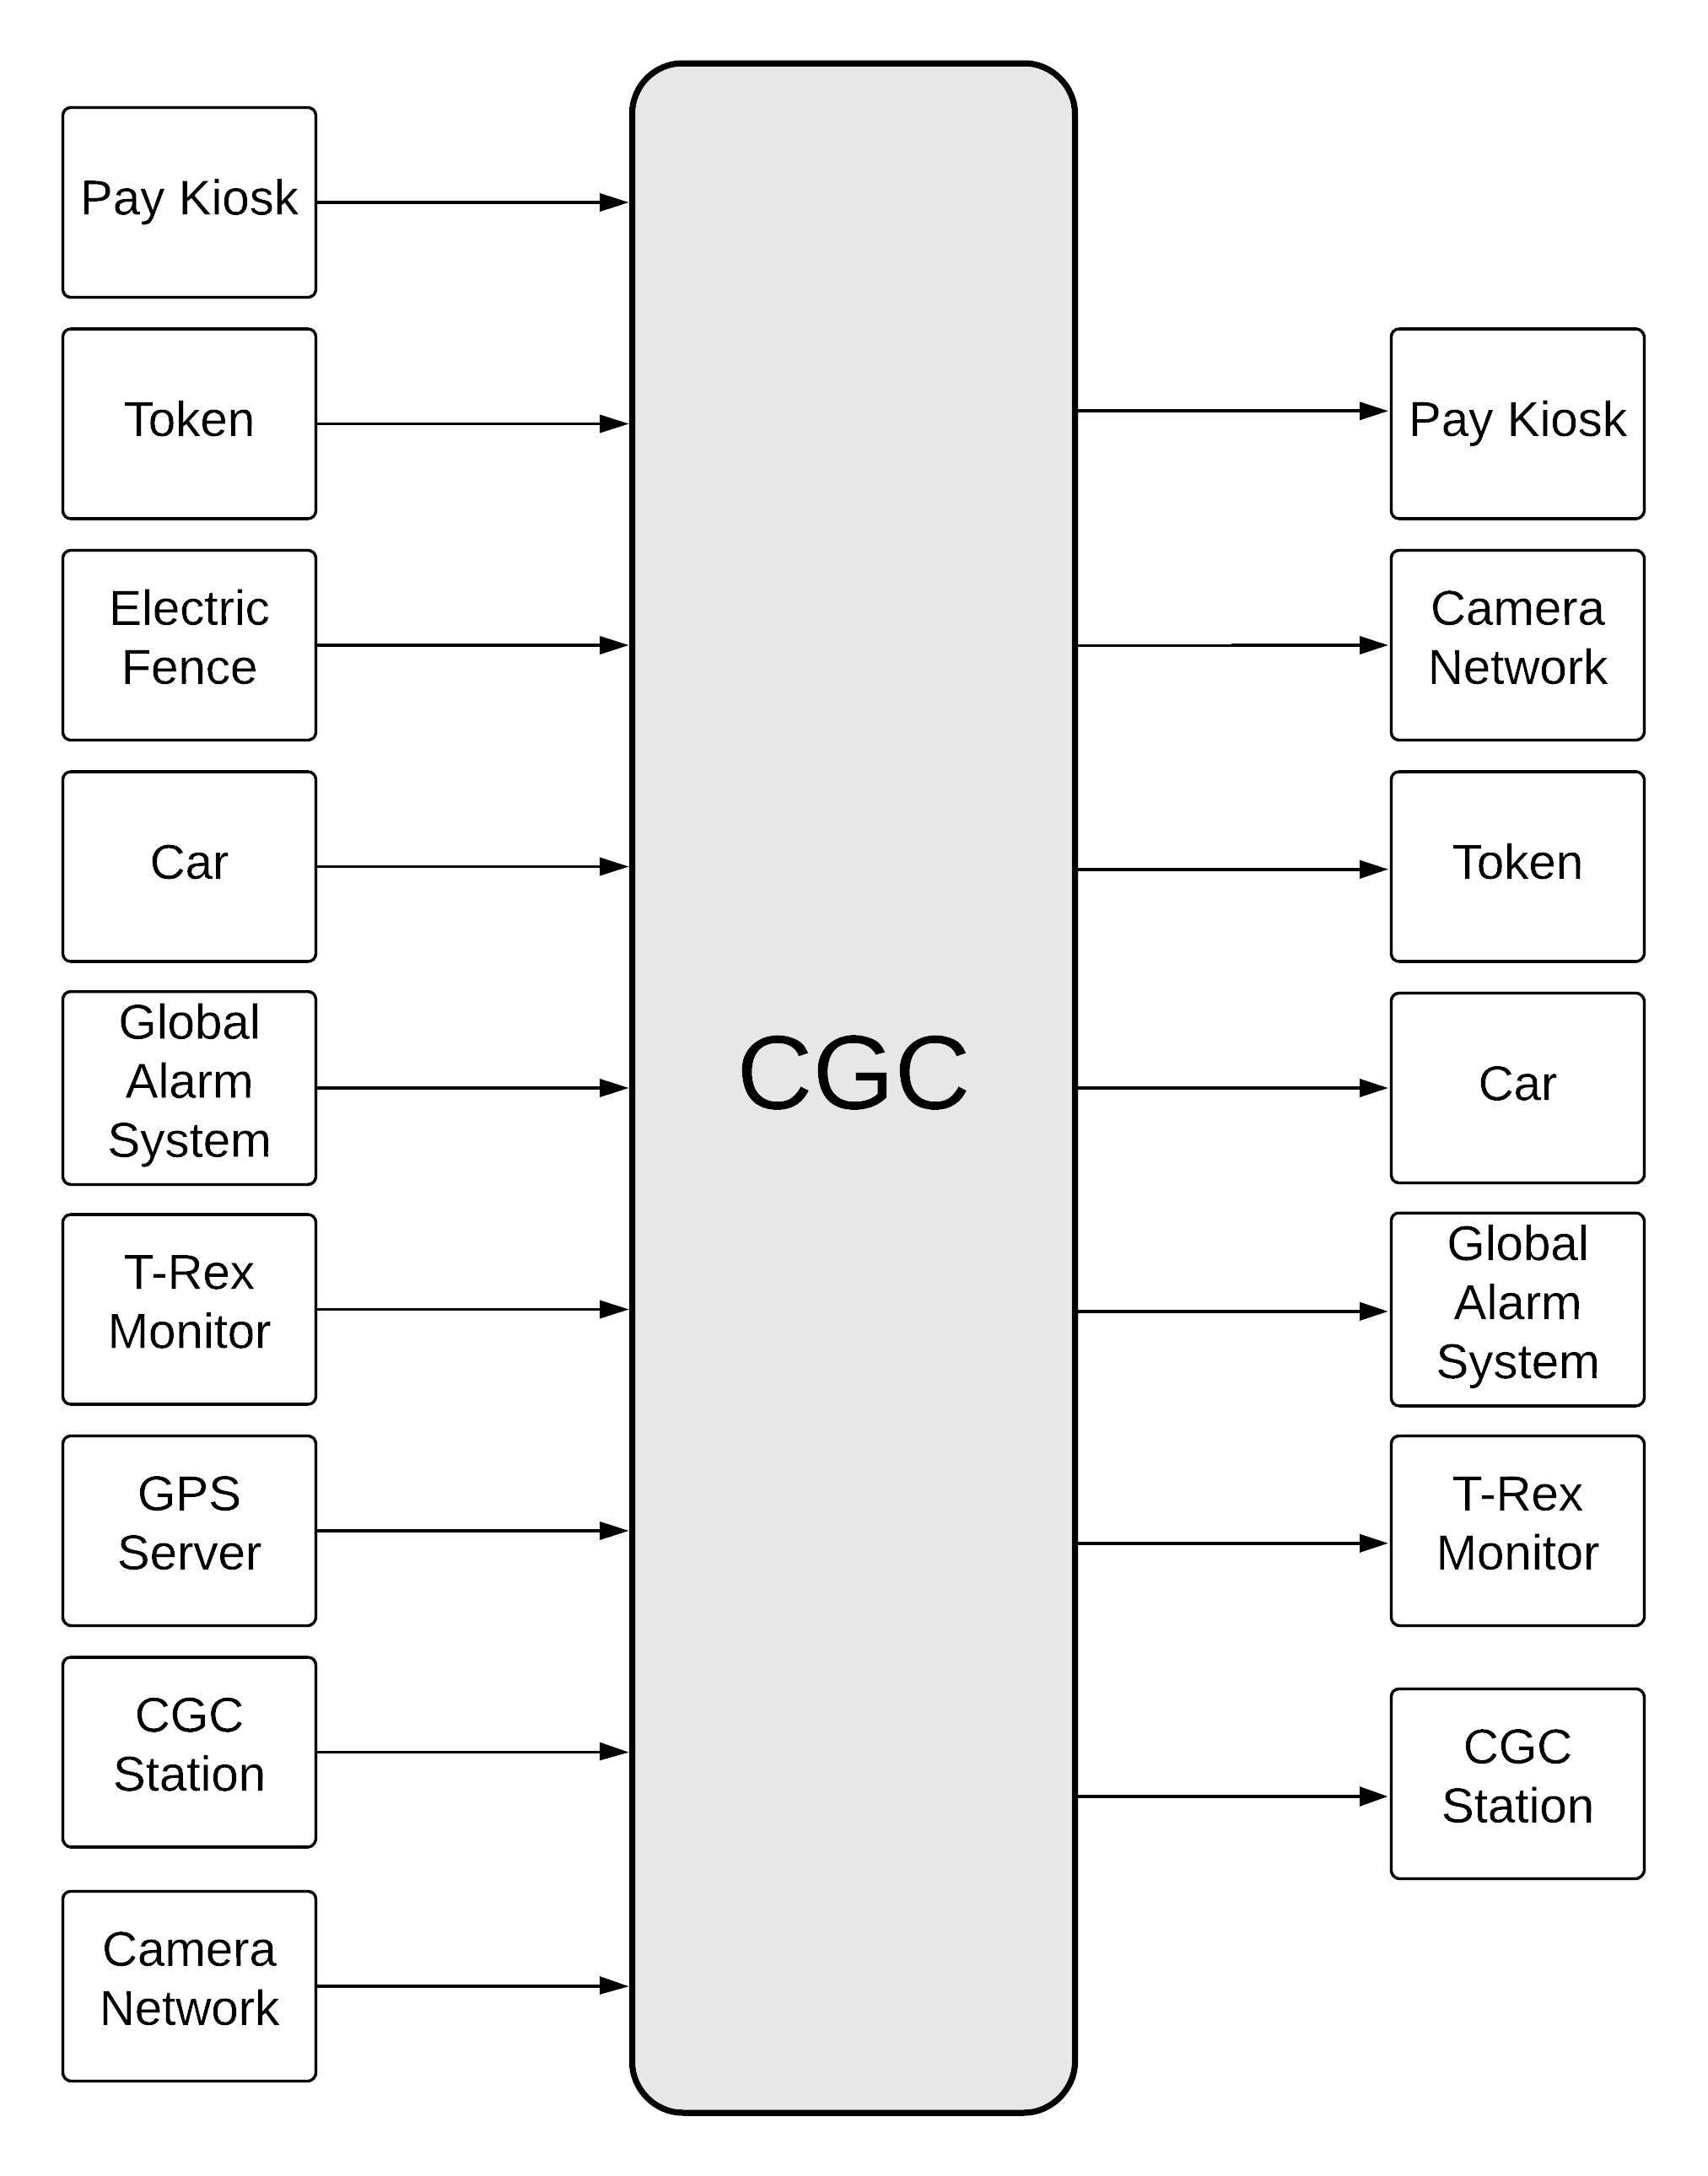
\includegraphics[scale=.20]{CGCBlackBox.png}}
  		\caption{A black box of high-level inputs and outputs of the \textit{CGCS}.}
  		\label{fig:blackbox}
	\end{figure}


\vfill
\pagebreak



\section{Interfaces} %Anas
\label{int}
%written by anas
\paragraph{} \textit{We have broken our interfaces\footnote{Interfaces by Siri and Anas.} up into main systems. these interfaces may be composes of their own sensors but they do not interface with the CGCS. The following list of interfaces list their sensors, hardware, and features.}

\subsection{Pay Kiosks}
	\paragraph{} \textit{The purpose of the the Pay Kiosk interface is to connect the physical Pay Kiosks to the CGCS. It is composed of sensors and is designed to do specific feature.}
		\subparagraph{Sensors}
			\begin{list}{}{}
					\item \textbf{Touch Screen: }used to sense user interaction. 
					\item \textbf{Credit card: }accepts all major credit/debit cards. 
					\item \textbf{Cash receptacle: }accepts and analyzes cash. 
			\end{list}
		\subparagraph{Hardware}
			\begin{list}{}{}
					\item \textbf{Change dispenser: }dispenses appropriate change to the visitor buying a token.
					\item \textbf{Token dispenser: }dispenses token with unique ID to user.
			\end{list}
		\subparagraph{Features}
			\begin{list}{}{}
					\item \textbf{Token builder: }this features will take the payment and the filled out user form and build a unique token for the visitor.
					\item \textbf{Maintenance: }this feature will let the employees manage certain issues associated with the pay kiosks and also will let the employees see the health of the machine. 
			\end{list}

\subsection{Token}
	\paragraph{} \textit{The Token will act as an interface to multiple systems. It will provide valuable information about the visitor and also interact with the visitor. }
		\subparagraph{Sensors}
			\begin{list}{}{}
					\item \textbf{Touch Screen: }used to interact with the users. 
					\item \textbf{GPS: }the Token will contain a GPS to sense the location of the token.
 
			\end{list}
		\subparagraph{Hardware}
			\begin{list}{}{}
					\item \textbf{RFID: }the RFID chip will be programmed with a unique ID and used for multiple purposes included access to various systems and areas.
					\item \textbf{Speaker: }the token contains speakers as hardware for alerts and instructions.
			\end{list}
		\subparagraph{Features}
			\begin{list}{}{}
					\item \textbf{Location/Map: }utilizes the GPS to provide location services.
			\end{list}

\subsection{Car}
	\paragraph{} \textit{There will be an interface with all the cars. The autonomous car will be built utilizing a partner. We will work closely with them to provide access to specific sensors and features.}
		\subparagraph{Sensors}
			\begin{list}{}{}
					\item \textbf{RFID reader: }that covers the proximity of the car and is used to grant access and count how many tokens are currently in the car. 
					\item \textbf{Seat Weight Sensor: }used to determine if there is someone sitting in the seat. 
					\item \textbf{Camera: }used by the car for autonomous driving and also connects to CGCS for a needed scenario. 
					\item \textbf{Mic: }used to sense voice for use in an intercom.
			\end{list}
		\subparagraph{Hardware}
			\begin{list}{}{}
					\item \textbf{Speaker: }used to alert guests.
					\item \textbf{Automatic Door Locks: }this will be initiated when the car is determined to be moving.
					\item \textbf{Wireless networking: }for communication purposes to communicate with the CGCS.
			\end{list}
		\subparagraph{Features}
			\begin{list}{}{}
					\item \textbf{Maintenance System: }allows for health checks and health status communication of the car.  
			\end{list}

% \section{Capabilities} %Zeke
% \label{cap}
% \textit{Herein is the outline of what the Elevator Control System will be capable and of what it will not be capable. Most of its capabilities may be described in terms of various protocols and its limitations may be described relative to the capabilities of external hardware that is to provide it data. For example, the \textit{ECS} should be expected to move cabins from floor to floor at safe speeds and accelerations but it cannot possibly account for speedometers and accelerometers that provide it inaccurate data. Sensors are assumed to not be faulty, as they are not part of the \textit{ECS} but are to provide it information.}
% % the outline for a solution
% \subsection{Capacity Protocol} The \textit{ECS}, under the assumption that all weight capacity sensors in the cabins are fully functional, may be expected to never provide service to a cabin whose weight capacity has been reached or exceeded. The cabin is to
% \begin{enumerate}
% \item Alert passengers of overcapacity issue.
% \item Notify passengers that it will not provide service until the issue has been resolved.
% \item Remain on the floor until the issue has been resolved.
% \item Continue regular functions after the issue has been resolved.
% \end{enumerate}

% \subsection{Emergency Protocol} The \textit{ECS}, under the assumption that the alarm system is fully functional, may be expected follow the correct protocol when presented with an emergency situation.
% \begin{enumerate}
% \item Close all doors (provided there are no obstructions).
% \item Move all cabins to the lobby floor without stopping at any floors between its initial floor and the lobby.
% \item Open all doors after having arrived to the lobby.
% \item Remain open until an emergency key is detected in the emergency keyhole.
% \end{enumerate}

% \subsection{Efficient Usage Protocol} The \textbf{ECS} may be expected to optimize resource usage in the following ways.
% \begin{enumerate}
% \item Any requests from floors between an elevator's \textit{current floor} and its most recent \textit{target floor} will be fulfilled so as to not waste time and energy by addressing requests in the order they were received.
% \item \label{mor} If more than one request is detected at the same time and the elevator is \textit{empty}, the \textit{ECS} will dispatch whichever elevator is closest to either \textit{target floor}.
% \item \label{eql} In the event that multiple requests are made simultaneously, that the elevator is \textit{empty} and that no \textit{target floor} is closer than another, the \textit{ECS} will arbitrarily break any ties by randomly choosing which elevator to dispatch to the floors.
% \item Any \textit{non-empty} elevators found to be in either situation \ref{mor} or \ref{eql} will ignore requests from floors located opposite of its direction.
% \item If a cabin is currently \textit{empty}, then the cabin will be allowed to travel at greater accelerations and speeds than when it is \textit{non-empty}.
% \end{enumerate}

% \subsection{Executive Usage Protocol} The \textit{ECS}, under the assumption that all \textit{executive keyholes} and \textit{executive keys} function properly, may be expected to only permit access to the penthouse when the correct key is inserted and detected in the correct keyhole by the ECS. The penthouse is also known as the topmost floor, floor 20, 20th floor, or executive suite.

% \subsection{Obstruction Protocol} The \textit{ECS}, under the assumption that all \textit{obstruction sensors} function properly, within all cabins and all bays, may be expected to never close any cabin doors nor any bay doors that find themselves obstructed. In the event that an obstruction is found, the \textit{ECS} shall
% \begin{enumerate}
% \item Stop all door motion in the associated cabin(s) and bays(s).
% \item Slowly decelerate the associated cabin(s) to a halt if in motion upon detection.
% \item Slowly open both sets of doors (away from the center of the cabin and bay openings).
% \item Remain open until the obstruction has been cleared.
% \item Continue regular service.
% \end{enumerate}

% \pagebreak
% \section{Design Constraints} %Matt
% \label{con}
% %restrictions placed on the solution space
% \paragraph{} \textit{The various requirements for the elevator control system are as follows}
% \subsection{General Constraints}
% \begin{itemize}
% 	\item The \textit{ECS} will service 20 floors.
% 	\item The \textit{ECS} will control four identical elevators.
% 	\item Each elevator bay will have one set of directional buttons.
% 	\item The bays on floor 20 will have only \textit{down} buttons.
% 	\item The bays on floor one will have only \textit{up} buttons.
% 	\item Each cabin will have one set of buttons, numbered for each floor.
% 	\item Each cabin will have two keyholes: EMERGENCY and EXECUTIVE.
% 	\item An elevator will only go to the top floor if an executive key is detected.	
% \end{itemize}
% \subsection{Safety Constraints}
% \begin{itemize}
% 	\item A weight sensor will be used to ensure capacity is not exceeded.
% 	\item The \textit{ECS} will have a two-phase emergency mode triggered by the fire alarm sensor.
% 	\item Neither the floor nor the cabin door can close while obstructed. There are sensors built in to aid in this.
% 	\item The elevator weight capacity will be 25\% of its cabin weight \citep{krupp}.
% 	\item ASME A17.1, Section 2.27 Emergency Operation and Signaling Device regulation will be followed \citep{asme}.
% 	\item No elevator will exceed a safe speeds nor acceleration.
% 	\item Elevators can only open their doors if they are aligned with a floor.
% \end{itemize}
\bibliography{../../ReferenceMaterial/BibTeX/references}
% run latex, then bibtex, then quickbuild all on the tex file
\end{document}
